
\chapter*{Introduction}
\addcontentsline{toc}{chapter}{Introduction}
This project has been developed under the supervision of Prof. Cecilia Di Ruberto and PhD students Andrea Loddo and Lorenzo Putzu.

\bigskip


Blood is a body fluid deliver. It contains and transport many of the nutrients substances that the man and the other animals use to live. That we call blood is principally a fluid divided in two elements: blood cells and blood plasma. Normally an individual has around 5 Litre of blood. The plasma blood constitutes the 55\% of the total fluid. It is mostly water(92\% by volume) and contains proteins, glucose, mineral ions, hormones and blood cells themselves.\cite{website:wiki} Mainly the cells are red blood cells and white blood cells(WBCs). In this dissertation we going to focus on WBC especially we will study the shape of these last.
White blood cells, also called leukocytes, are the cells with the task of controlling the body against both infectious disease and foreign invaders. All leukocytes have a nucleus that distinguishes them by other blood cells, in particular red blood cells and platelets. The generic term leukocytes includes very different cells population: neutrophil, granulocytes, basophilic granulocytes and eosinophilic granulocytes. This set of three categories is defined as   polymorphonucleated granulocytes. The other set that includes monocytes and lymphocytes is defined agranulocytes mononuclear. In a nutshell leukocytes are dived in these two sets by the nuclei shape.\ref{fig:kindLeuko}
\begin{figure}
	\begin{center}
		\centering
		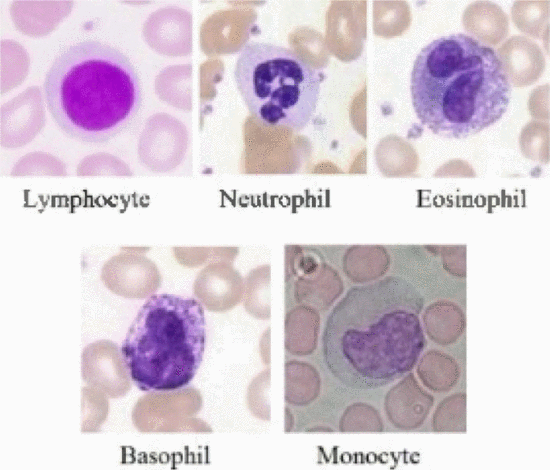
\includegraphics[scale=0.5]{img/leuko.png}
		\caption{Example of the different kind of leukocytes\cite{ann17}}
		\label{fig:kindLeuko}
	\end{center}
\end{figure}

\section*{White blood cells segmentation}
Segment an image means divide an image in regions of interest. It's used to obtain a more compact image that it is used to extract objects or to analyse an image. More precisely, image segmentation is the process of assigning a label to every pixel in an image such that pixels with the same label share certain visual characteristics. In this case the main feature is to find edges and white blood cells nuclei. At a first look it seems a banal problem, because the we think that every single cell is strongly separated by the others, but obviously it is the best case that we can find. Commonly the microscope photos that we analyse contains noise and in particular the leukocytes overlaps both others leukocytes and red blood cells. For these reasons segment leukocytes is still an unresolved problem. As explain above there are 2 class of leukocytes that are dissimilar by the nuclei shape. This is an high problem because if the solution to find all the white blood cells was based on the search of circular shapes, it's trivial that it will be impossible to recognize a granulocytic from a monocyte.


\bigskip


There are a lot of heuristics and approaches that try to divide white blood cells. This dissertation proposes a new approach of pure segmentation using the Vector Field Convolution, in particular tries to find a division between the overlaps between the cells. The used dataset is ALL-IDB dataset, a public dataset created by the University of Milan. It contains microscopic images of blood samples, specifically designed for the evaluation and the comparison of algorithms for segmentation and image classification.


\bigskip 


We choose this vector field because the common practice to extract the features by the images utilizes thresholds, but what happens if the image has a low definition and all the cells are in overlap with their? Using that field to describe the image is possible to transcend by the shape of the features and focus themselves on the points that have a non-uniform virtual field. This technique then considers only the points that describe the edges of the white blood cells. After the image elaboration the result is an image that contains only segmented leukocytes. With this result we can label every cell without human work.


\bigskip


The first step of the algorithm pre-processes the image in order to overcome the non-linearity  of colour distribution inside the image. The literature says that we can overtake this problem using the mean-shift model. The second step applies the Vector Field Convolution on the edge image obtained by the first step, in order to obtain an intensity image of the cells. The third step focuses is work on the extraction of the angle image in order to obtain the direction of each pixel and to apply to it the Energy function. The fourth step applies the median filtering to the energy image and the angle image and puts them in overlay in order to apply the skeleton function after an opening of the closing of the image. After this step we obtain, joining the skeleton image with the black and white leukocytes image and the Energy image, the first result: the segmentation of the cells and in particular also the segmentation of the cells in overlap.
The fifth step merges all the little image's imperfections in order to count the cells and to have a perfect segmentation of the cells.